\documentclass{beamer}		% This tells LaTeX the document will be a "beamer" presentation

\usetheme{Madrid}		% Sets basic formatting.  Lots of options, google "beamer themes"
\usepackage[ruled,vlined]{algorithm2e}
\usecolortheme{dolphin}	% Sets the colour scheme.  Lots of options, google "beamer color themes"

\setbeamertemplate{navigation symbols}{}	% Manually changes one piece of formatting.  See what the difference is by commenting this line out.

\date{\today}	% Insert the date of your presentation. \today gives an unsurprising automatic date.

\title[Adversarial Examples]{Adversarial Examples\\for Eye-State Classification}	% Insert your title.  Depending on the theme you choose above, a "short title" might be useful, as it will appear on the footer of each slide.

\author[Şefika]{Şefika EFEOĞLU} % Insert your name

\institute{University of Potsdam} % Self-explanatory

\begin{document} 	% Let's begin

% Presentations come in slide frames.  You have to tell LaTeX when to start a frame, and when to end the frame.  The most common error beginners make with beamer is forgetting the \end{frame} command.	

\begin{frame}	

\titlepage	% Prints a title page populated with the information given in the preamble

\end{frame}		
\begin{frame}{Motivation}
   \begin{figure}[!htb]

   \begin{minipage}{0.48\textwidth}
     \centering
     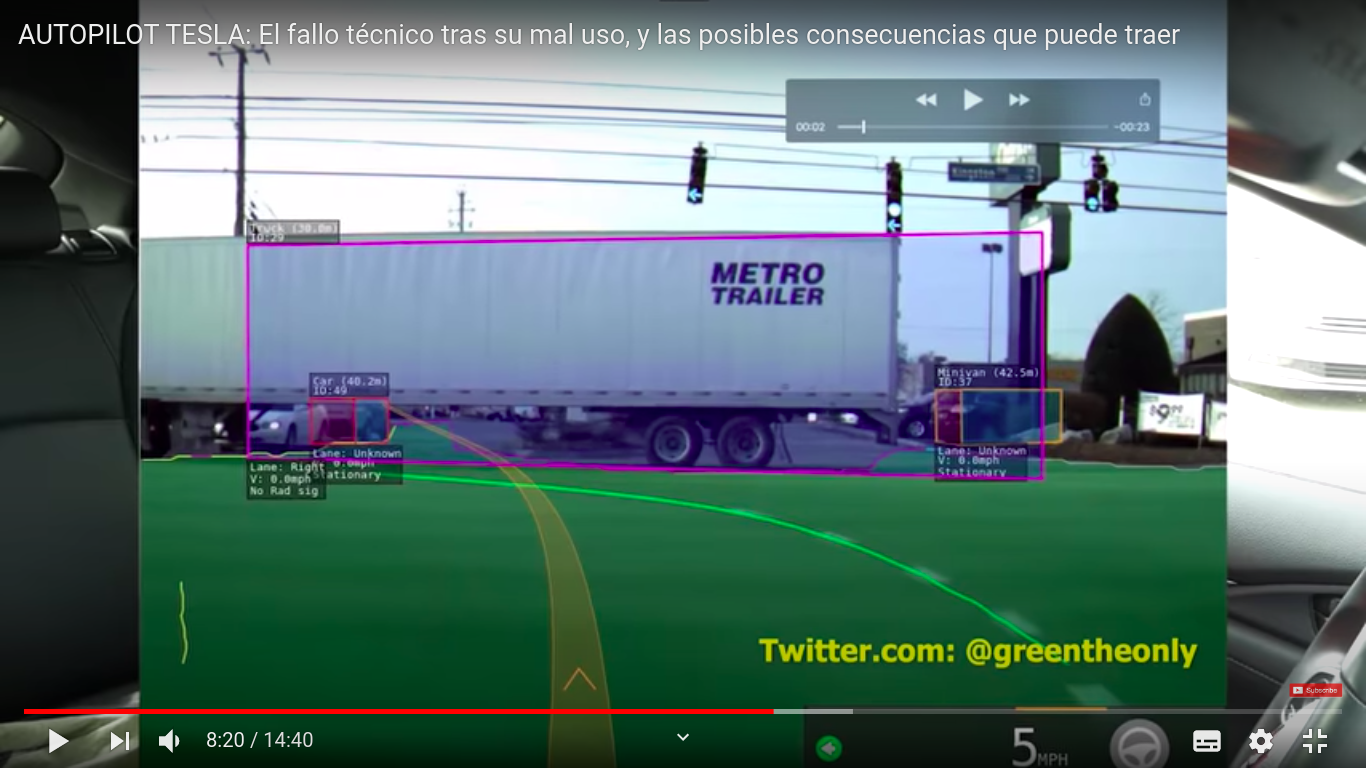
\includegraphics[height=4cm,width=.9\linewidth]{Adversarial_examples_Tesla.png}
   
   \end{minipage}\hfill
   \begin{minipage}{0.48\textwidth}
     \centering
     \includegraphics[height=3cm,width=.9\linewidth]{aa}
 
   \end{minipage}
\end{figure}
\end{frame}
\begin{frame}{Motivation Continue..}
     \begin{figure}
        \centering
        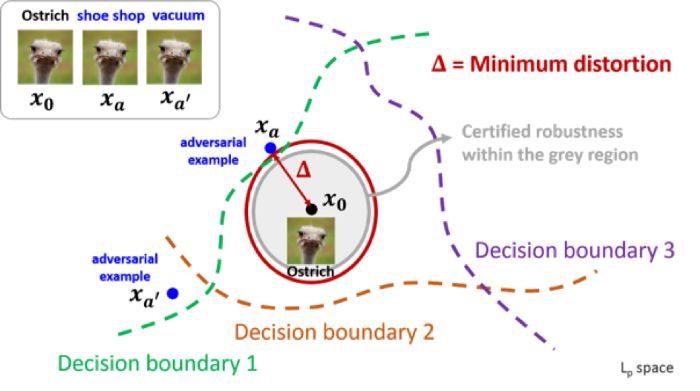
\includegraphics[height= 5 cm] {robustness.png}
    \end{figure}
\end{frame}

\begin{frame}{Overview}	
\begin{itemize}
\item Introduction
\item Background Knowledge
\item Methodologies
\item Results
\item Conclusion
\item Bibliograph
\end{itemize}
\end{frame}	

\begin{frame}{Introduction}	
\begin{itemize}
\item Neural Networks achieves extreme accuracy on image classification tasks
\item but are vulnerable to adversarial examples.
\item Regularization is ineffective
\item Current approaches:
\end{itemize}
Contribution: regularization-based approach to adversarial examples
Objective: Improve the robustness of Eye-State Classifier using Adversarial Examples
\end{frame}	
\begin{frame}{Background Knowledge}	
\begin{enumerate}
    \item Adversarial Examples
    \item Fast Gradient Sign Method
    \item  Wide Residual Networks
    \item Parseval Networks
    \item Signal to Noise Ratio (SNR)
\end{enumerate}
\end{frame}	


\begin{frame}{Adversarial Examples}
\begin{columns}
\column{0.5\textwidth}
\begin{enumerate}
\item specialised inputs created with 
the purpose of confusing a neural network
\item misclassification
\item fools the networks identifying a given input
\end{enumerate}
\column{0.5\textwidth}
Types of adversarial attack
\begin{enumerate}
    \item Blackbox attack
    \item WhiteBox Attack
    \begin{itemize}
        \item Fast Gradient Sign Method
        \item Projected Gradient Descent
        \item Deepfool
        so on..
    \end{itemize}
    
\end{enumerate}
\end{columns}
\begin{figure}
    \centering
    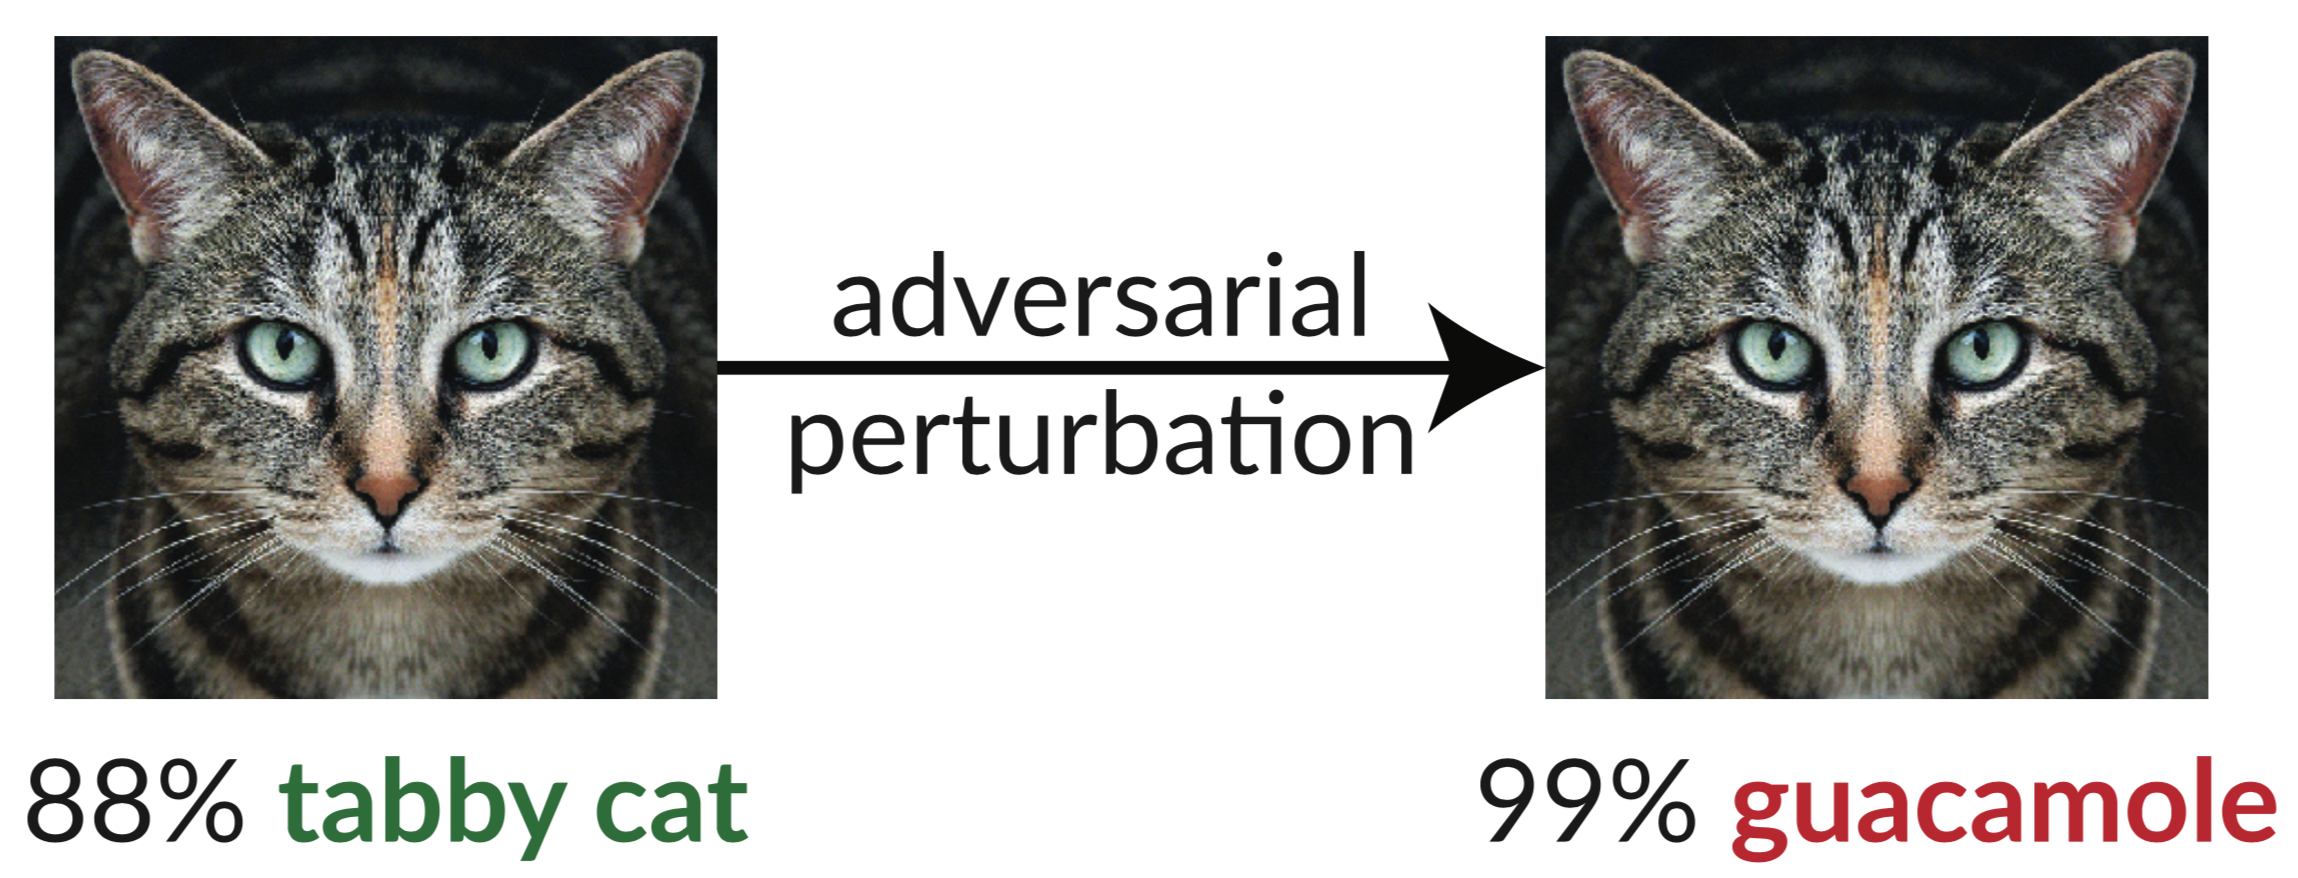
\includegraphics[height=3 cm]{example_adversarial_examples.png}
    \caption{adversarial example of the cat image}
\end{figure}

\end{frame}	
\begin{frame}{History of Adversarial Examples}	
\begin{figure}
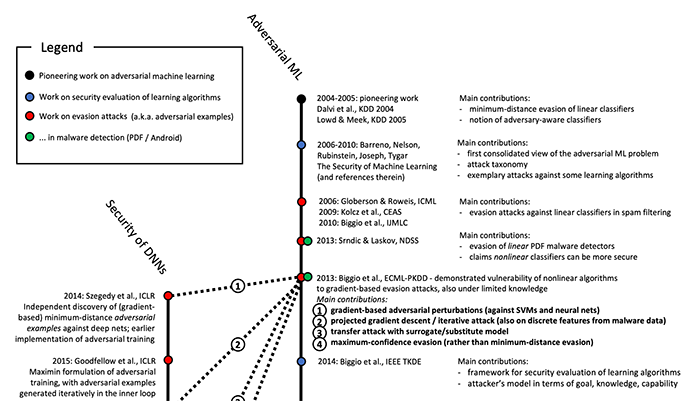
\includegraphics[height=7cm]{basic_image_adversaries_history.png}
\caption{History of Adversarial Examples}
\end{figure}
\end{frame}	
\begin{frame}{Fast Gradient Sign Method}	
\begin{definition}
\[
adv_x = x+\epsilon \cdot sign(\bigtriangledown _{x}J(\theta ,x,y))
\]
\end{definition}
\begin{figure}
    \centering
    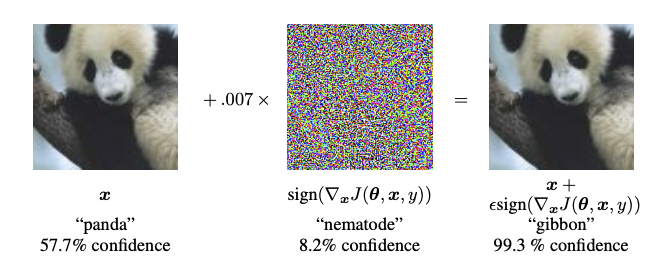
\includegraphics[height=4cm]{adversarial_example.png}
    \caption{the example of that how adversarial example of an image is obtained using Fast Gradient Sign Method}
\end{figure}
\end{frame}	

\begin{frame}{Wide Residual Network}
\begin{block}{Problem of Deep Neural Networks}
\begin{itemize}
    \item improved accuracy costs is expensive
    \item training is a problem of diminishing feature reuse
    \item very slow to train
\end{itemize}
\end{block}
\pause
\begin{block}{Proposed solutions}
\begin{itemize}
  \item decrease depth
  \item increase width of residual networks(Wide ResNet).
\end{itemize}
\end{block}
\end{frame}
\begin{frame}{Wide Residual Network-Residual Blocks}
\begin{figure}	% for graphics
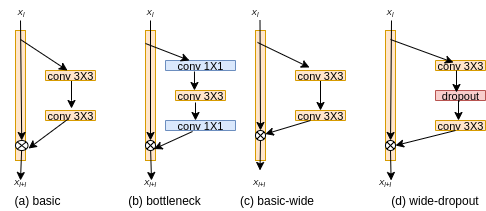
\includegraphics[height=4cm]{Model-WideResNet.png}
\caption{Various Blocks}
\end{figure}
\end{frame}	
\begin{frame}{Parseval Networks}	
\begin{block}{Objectives}
Using the advantages of orthogonality and convexity constraint in aggregation constraints, improve the accuracy of the deep neural networks. Luckily, it provides faster converges on learning curves.
\end{block}
\pause
2 constraints below and parseval training are considered
\begin{itemize}
\item Orthogonality Constraint
\item Convexity Constraint in Aggregation Layer
\item Parseval Training
\end{itemize}
\end{frame}	

\begin{frame}{Orthogonality Constraint}
\begin{definition}
\begin{itemize}
    \item an optimization algorithm on the manifold of orthogonal matrices
    \item another name is Stiefel Manifold
    \item \[R_{\beta}\left ( W_{k} \right )\leftarrow \frac{\beta}{2}\left | \left |W _{k}^{T}W_{k} - I \right | \right |_{2}^{2}\]is expensive after each gradient update step.
    \item after every main gradient update, second update is applied to make the algorithm more efficient
\end{itemize}
\end{definition}
\pause
\[W_{k}\leftarrow (1+\beta )W_{k}-\beta W_{k}W_{k}^{T}W_{k}\]

\end{frame}	
\begin{frame}{Convexity Constraint in Aggregation Layer}
\begin{definition}
\begin{itemize}
    \item In Parseval Networks, aggreagtion layers output a convex combination of their inputs.
    \item To ensure that Lipschitz constant at the node n is such that\[ \Lambda _{p}^{n}\leq 1\]
    euclidean projection is applied below
\end{itemize}

\end{definition}
\[\alpha^{*}=\arg \min _{\gamma \in \Delta ^{K-1}}\left | \left | \alpha-\gamma \right | \right |_{2}^{2}\]
\end{frame}
\begin{frame}{Parseval Training}
\scriptsize

\begin{algorithm}[H]
\SetAlgoLined
 \Theta = \left \{ W_k, \alpha_{k} \right \}_{K}^{k=1}, e\leftarrow 0 \;
 
 \While {\left \{ e \leq E \right \}}{
  Sample a minibatch \left \{ \left ( x_i, y_i \right ) \right \}_{i=1}^{B}.\;
  
  \For {k \in \left \{ 1,...,K \right \}}{

    Compute the gradient \;
    G_{W_{k}} \leftarrow \bigtriangledown_{W_{k}} \mathit{l} (\Theta, \left \{ (x_i, y_i) \right \})\
    
    G\alpha_{k} \leftarrow \bigtriangledown_{\alpha_{k}} \mathit{l}(\Theta, \left \{ (x_i, y_i) \right \})
    
    Update the parameters:
    
    W_{k} \leftarrow W_{k} - \epsilon \cdot  G_{w_{k}}
    
    \alpha_{k} \leftarrow \alpha_{k} - \epsilon \cdot  G_{\alpha_{k}}\;
    
    \If{hidden layer}{
    Sample a set S of rows of W_{k}\.
    
    Projection:
    
    W_{s} \leftarrow (1+\beta)W_{s}- \betaW_{s}W_{s}^{T}W_{s}.
    
    \alpha_{k} \leftarrow argmin_{\gamma \in \Delta ^{K-1}}\left | \left | \alpha_{K-\gamma} \right | \right |_{2}^{2}
    
    
   }
  }
  
  e \leftarrow e+1
  
 }
 \caption{Parseval Training}
\end{algorithm}
\end{frame}

\begin{frame}{Signal to Noise Ratio (SNR)}	
\begin{enumerate}
    \item abbreviated as SNR or S/N)
    \item a measure used in science and engineering 
    \item the ratio of useful information to false or irrelevant data in a conversation or exchange.
\end{enumerate}
 \[
SNR(x,\delta _{x}) = 20\log_{10}\frac{\left \| x \right \|_{2}}{\left \| \delta _{x} \right \|_{2}}
\]
\begin{figure}
    \centering
    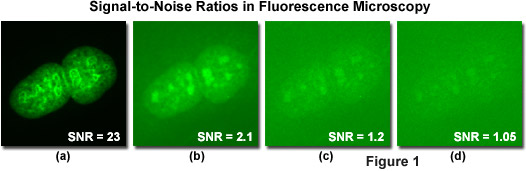
\includegraphics[height = 3cm]{signaltonoise.jpg}
    \caption{Example}
    \label{fig:my_label}
\end{figure}
\end{frame}	
\begin{frame}
\frametitle{Methodologies}
\begin{figure}	% for graphics
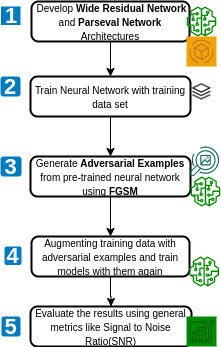
\includegraphics[height=7cm]{Model-Page-2.png}
\caption{Flowchart of the Project}
\end{figure}
\end{frame}	
\begin{frame}
\frametitle{Eye-State Data Set}
\begin{figure}
    \centering
    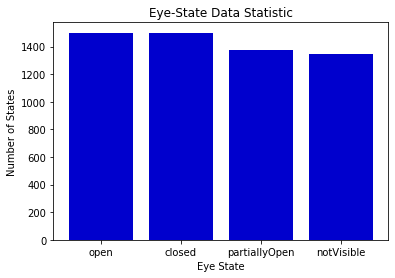
\includegraphics[height=4 cm]{data_histogram.png}
    \caption{Eye-State data set consists of 5400 images, and the distribution of each eye state on the histogram }
\end{figure}
\end{frame}
\begin{frame}
\frametitle{Wide Residual Network vs Parseval Network}
\begin{table}
\begin{tabular}{l | c | c }
Properties Name & Wide Residual Networks & Parseval Networks\\
\hline \hline
Kernel Initializer & Gaussian & Uniform \\ 
Orthoganality Constraint & No & Yes\\
Lipschitz Constant & No & Yes\\
\end{tabular}
\caption{shows that the properties of two different networks}
\end{table}
\end{frame}	

\begin{frame}{Neural Network Structure}
\begin{table}

\begin{tabular}{l | c | c}\hline \hline
groupp name & output size & block type = B(3,3)&&\\
\hline
conv1 & 32 x 32 & [3x3, 16] &&\\ 
conv2 & 32 x 32 & \[ \begin{bmatrix}
3x3, 16 x k\\ 
3x3, 16 x k
\end{bmatrix}\] x N &&\\

conv3 & 16 x 16 &\[ \begin{bmatrix}
3 x 3, 32 x k\\ 
3 x 3, 32 x k
\end{bmatrix}\] x N&&\\

conv4 & 8 x 8 &\[ \begin{bmatrix}
3x3, 64 x k\\ 
3x3, 64 x k
\end{bmatrix}\] x N&&\\

avg-pool & 1 x 1 & [8 x 8] &&\\
\hline
\end{tabular}
\caption{Structure of Wide Residual Blocks}
\end{table}
\end{frame}

\begin{frame}{Hyperparameter Tuning}
\begin{table}
\begin{tabular}{l | c |c|c}
Properties Name & Width(k)  & Accuracy && Loss &&\\
\hline \hline
Baseline of Simple ResNet & 1 & 0.667830 && 0.942042&&\\ 
Baseline of Wide ResNet & 2 & 0.656195 && 1.077292&&\\
WideResNet16-4 & 4 & 0.641070 && 1.374967 &&\\
\end{tabular}
\caption{shows the effect of width factor on deep neural networks which has 16 layers.}
\end{table}
\end{frame}

\begin{frame}{Non-Adversarial Training Results}
\begin{figure}[!htb]

   \begin{minipage}{0.48\textwidth}
     \centering
     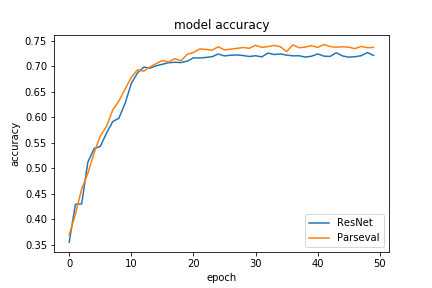
\includegraphics[height=4cm,width=.9\linewidth]{NonAdversarialTraining_accuracy.png}
     \caption{Simple ResNet and Parseval}
   \end{minipage}\hfill
   \begin{minipage}{0.48\textwidth}
     \centering
     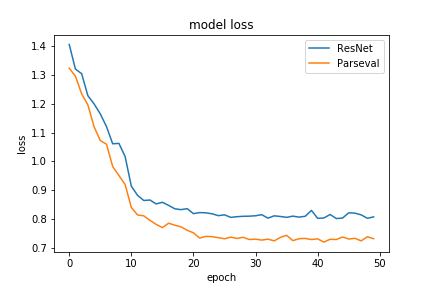
\includegraphics[height=4cm,width=.9\linewidth]{NonAdversarialTraining_loss.png}
     \caption{Simple WideResNet and Parseval}
   \end{minipage}
\end{figure}
\end{frame}
\begin{frame}{Attack the Model with Different Noise Levels}
   \begin{figure}[!htb]
    
   \begin{minipage}{0.48\textwidth}
     \centering
     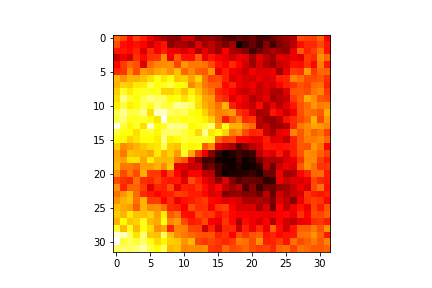
\includegraphics[height=4cm,width=0.9\linewidth]{OriginalImage.png}
      \caption{Label: Open}
   \end{minipage}\hfill
   \begin{minipage}{0.48\textwidth}
     \centering
     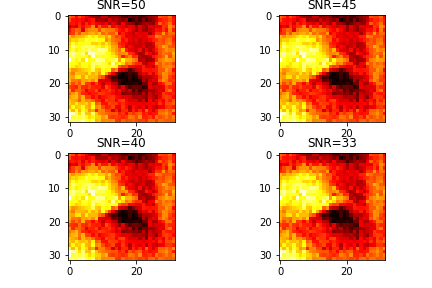
\includegraphics[height=4cm,width=0.9\linewidth]{PertubatedImagesforDifferentSNR.png}
     \caption{Label: Partly Open}
   \end{minipage}
\end{figure}
\end{frame}
\begin{frame}{Results of Adversarial Training}
\begin{figure}[!htb]
    
   \begin{minipage}{0.48\textwidth}
     \centering
     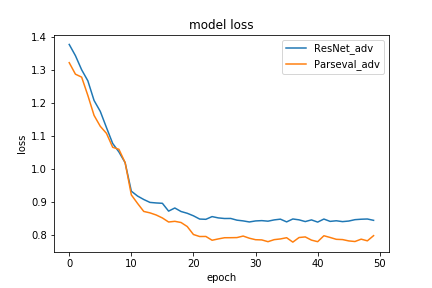
\includegraphics[height=4cm,width=.9\linewidth]{compare_ResNetvsParseval_adversarial_loss.png}
      \caption{Simple ResNet and Parseval of it.}
   \end{minipage}\hfill
   \begin{minipage}{0.48\textwidth}
     \centering
     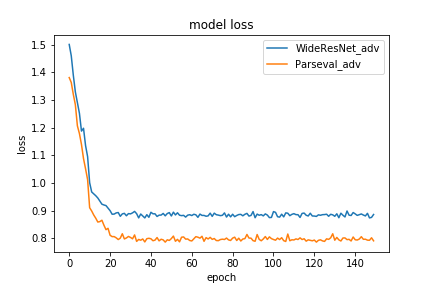
\includegraphics[height=4cm,width=.9\linewidth]{compare_ResNetvsParseval_adversarial_for_advanceModel_loss.png}
     \caption{Simple Wide Residual Network and Parseval of it.}
   \end{minipage}
\end{figure}
\end{frame}

\begin{frame}{Results of Adversarial Training}
\begin{figure}[!htb]
   \begin{minipage}{0.48\textwidth}
     \centering
     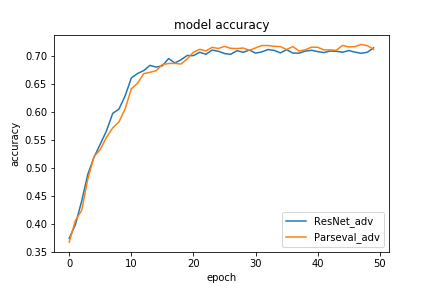
\includegraphics[height=4cm,width=.9\linewidth]{compare_ResNetvsParseval_adversarial_accuracy.png}
     \caption{Simple ResNet and Parseval ofit.}\label{Fig:Data1}
   \end{minipage}\hfill
   \begin{minipage}{0.48\textwidth}
     \centering
     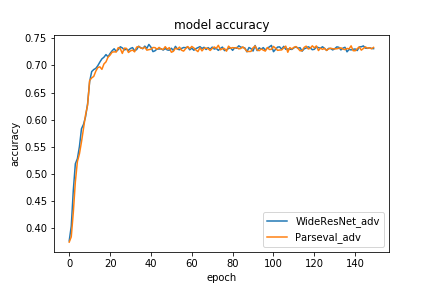
\includegraphics[height=4cm,width=.9\linewidth]{compare_ResNetvsParseval_adversarial_for_advanceModel_accuracy.png}
     \caption{Simple Wide Residual Network and Parseval of it.}\label{Fig:Data2}
   \end{minipage}
\end{figure}
\end{frame}
\begin{frame}{Signal To Noise Ratio Results}
\begin{figure}
    \centering
    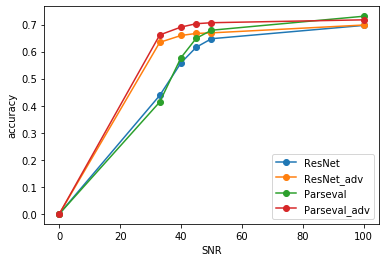
\includegraphics[height=5cm]{SNR.png}
    \caption{The accuracies of the models against different Signal to Noise Ratio (SNR)}
\end{figure}
\end{frame}

\begin{frame}{Conclusion}

\end{frame}



\begin{frame}{Bibliography}
\;

\end{frame}






\end{document}	% Done!